% !TEX TS-program = pdflatex
% !TEX encoding = UTF-8 Unicode

% This is a simple template for a LaTeX document using the "article" class.
% See "book", "report", "letter" for other types of document.

\documentclass[11pt]{article} % use larger type; default would be 10pt
\usepackage{graphicx}
\graphicspath{ {images/} }
\usepackage[utf8]{inputenc} % set input encoding (not needed with XeLaTeX)

%%% Examples of Article customizations
% These packages are optional, depending whether you want the features they provide.
% See the LaTeX Companion or other references for full information.

%%% PAGE DIMENSIONS
\usepackage{geometry} % to change the page dimensions
\geometry{a4paper} % or letterpaper (US) or a5paper or....
% \geometry{margin=2in} % for example, change the margins to 2 inches all round
% \geometry{landscape} % set up the page for landscape
%   read geometry.pdf for detailed page layout information

\usepackage{graphicx} % support the \includegraphics command and options

% \usepackage[parfill]{parskip} % Activate to begin paragraphs with an empty line rather than an indent

%%% PACKAGES
\usepackage{booktabs} % for much better looking tables
\usepackage{array} % for better arrays (eg matrices) in maths
\usepackage{paralist} % very flexible & customisable lists (eg. enumerate/itemize, etc.)
\usepackage{verbatim} % adds environment for commenting out blocks of text & for better verbatim
\usepackage{subfig} % make it possible to include more than one captioned figure/table in a single float
% These packages are all incorporated in the memoir class to one degree or another...

%%% HEADERS & FOOTERS
\usepackage{fancyhdr} % This should be set AFTER setting up the page geometry
\pagestyle{fancy} % options: empty , plain , fancy
\renewcommand{\headrulewidth}{0pt} % customise the layout...
\lhead{}\chead{}\rhead{}
\lfoot{}\cfoot{\thepage}\rfoot{}

%%% SECTION TITLE APPEARANCE
\usepackage{sectsty}
\allsectionsfont{\sffamily\mdseries\upshape} % (See the fntguide.pdf for font help)
% (This matches ConTeXt defaults)
\usepackage{amsmath}
\usepackage{systeme}
\usepackage{listings}

%%% ToC (table of contents) APPEARANCE
\usepackage[nottoc,notlof,notlot]{tocbibind} % Put the bibliography in the ToC
\usepackage[titles,subfigure]{tocloft} % Alter the style of the Table of Contents
\renewcommand{\cftsecfont}{\rmfamily\mdseries\upshape}
\renewcommand{\cftsecpagefont}{\rmfamily\mdseries\upshape} % No bold!

%%% END Article customizations

%%% The "real" document content comes below...

\title{CS770: Assignment 4}
\author{Ronghao Yang\\ID: 20511820}
%\date{} % Activate to display a given date or no date (if empty),
         % otherwise the current date is printed 

\begin{document}
\maketitle

\section{Question 1}
\subsection{Question 1a}
For cubic spline, let the function $S(x)$ define the spline function\\\medskip
\centerline{where $a = x_{0} < x_{1} < x_{2} < x_{3} < ......< x_{n} = b$}
 
\begin{equation}
  S(X)=\left\{
  \begin{array}{@{}ll@{}}
    S_{0}(x), & \text{}\ x_{0}<x<x_{1} \\
    S_{1}(x), & \text{}\ x_{1}<x<x_{2}\\
    ......\\
    S_{i}(x), & \text{} \ x_{i}<x<x_{i+1}\\
    ......\\
    S_{n-1}(x), & \text{}\ x_{n-1}<x<x_{n}
  \end{array}\right.
\end{equation} 
\centerline{Where each $S_{i}(x)$ has degree 3 in this case.}\\
In cubic spline, $S(x)$ satisfies
\[
\systeme*{
S_{i}(x_{i})=S_{i+1}(x_{i}),
S_{i}'(x_{i})=S_{i+1}'(x_{i}), 
S_{i}''(x_{i})=S_{i+1}''(x_{i}),
S_{i}(x_{i}) = y_{i}
}
\]
\centerline{Where each $i = 0, 1, 2, ......, n-2$}\\
By the definition of natural cubic spline, we have two additional constraints,
\[
\systeme*{
S_{0}''(x_{0})=0,
S_{n-1}''(x_{n-1})=0
}
\]
\subsection{Question 1b}
\begin{lstlisting}[language=Octave]
function [coeffs] = nSpline(X,y)
%This function returns the coefficients of the natural cubic spline
%X and y are the input points where f(X(i)) = y(i)
%Each spline function on each interval has degree 3

%Si = a+bx+cx^2+dx^3
%We have n such Si's, where is n = length(X)-1
%coeffs should be [a1;b1;c1;d1;a2;b2;.....;an;bn;cn;dn]
%coeffs is a 4n by 1 vector
    
    numP = length(X);
    %numP is the number of points
    n =numP - 1;
    %n is the number of spline functions
    
    K = [];
    %initialize the matrix to be empty
    A = [];
    %A contains all the known values
    %K*coeffs = A
    
    %we construct the matrix using for loop
    for i = 1:numP
        a = (i-1)*4+1;
        b = a+1;
        c = b+1;
        d = c+1;
        %a,b,c,d are indices for the convinience of calculation
        %a,b,c,d indicate the next polynomial
        %to access the previous polynomial
        %use a-4, b-4, c-4, d-4
        
        if i==1
            tempK = zeros(1,4*n);
            tempK(1,c) = 2;
            tempK(1,d) = 6*X(i);
            K = [K;tempK];
            A = [A;0];
            tempK = zeros(1,4*n);
            tempK(1,a) = 1;
            tempK(1,b) = X(i);
            tempK(1,c) = X(i)^2;
            tempK(1,d) = X(i)^3;
            K = [K;tempK];
            A = [A;y(i)];
        end
        
        
        if i==numP
            tempK = zeros(1,4*n);
            tempK(1,c-4) = 2;
            tempK(1,d-4) = 6*X(i);
            K = [K;tempK];
            A = [A;0];
            tempK = zeros(1,4*n);
            tempK(1,a-4) = 1;
            tempK(1,b-4) = X(i);
            tempK(1,c-4) = X(i)^2;
            tempK(1,d-4) = X(i)^3;
            K = [K;tempK];
            A = [A;y(i)];
        end
        %these the special end points contraints for natural cubic constraint
        
        if i>1 && i<numP
            tempK = zeros(1,4*n);
            tempK(1,a-4) = 1;
            tempK(1,b-4) = X(i);
            tempK(1,c-4) = X(i)^2;
            tempK(1,d-4) = X(i)^3;
            K = [K;tempK];
            A = [A;y(i)];
            tempK = zeros(1,4*n);
            tempK(1,a) = 1;
            tempK(1,b) = X(i);
            tempK(1,c) = X(i)^2;
            tempK(1,d) = X(i)^3;
            K = [K;tempK];
            A = [A;y(i)];
        end
        %this is the constraint for S(xi) = yi
        
        if i>1 && i<numP
            tempK = zeros(1,4*n);
            tempK(1,b-4) = 1;
            tempK(1,c-4) = 2*X(i);
            tempK(1,d-4) = 3*X(i)^2;
            tempK(1,b) = -1;
            tempK(1,c) = -2*X(i);
            tempK(1,d) = -3*X(i)^2;
            K = [K;tempK];
            A = [A;0];
            %this is the constraint for Si'(xi) = Si+1'(xi)
            
            tempK = zeros(1,4*n);
            tempK(1,c-4) = 2;
            tempK(1,d-4) = 6*X(i);
            tempK(1,c) = -2;
            tempK(1,d) = -6*X(i);
            K = [K;tempK];
            A = [A;0];
            %this is the constraint for Si''(xi) = Si+1''(xi)
        end
    end
    
    coeffs = K\A;
    
end
\end{lstlisting}

This code has been proven to run correctly, the results for Question 4 was obtained using this function.

\section{Question 2}
For an interpolating polynomial $P$, it can be expressed as\\\\
\centerline{$P(x)$ = $a_{0}p_{0}(x)+a_{1}p_{1}(x)+a_{2}p_{2}(x)+......+a_{n-1}p_{n-1}(x)$}\\\\
In this question, we have four give points $(-1,-5)$, $(0,1)$, $(1,1)$, $(2,1)$
\subparagraph{• Monomial Basis}\mbox{}\\
For monomial basis, we have\\ 
\centerline{$p_{i}(x)$ = $x^{i-1}$, for $i$ = $1,2,...,n$}
Since we have four points here, the interpolating polynomial should have form of\\
\centerline{$P(x)$ = $a_{0} + a_{1}x+ a_{2}x^{2} + a_{3}x^{3}$}\\
By applying matrix calculation, we get\\
\centerline{$a_{0}=1\;\;a_{1}=2\;\;a_{2}=-3\;\;a_{3}=1$}\\
\centerline{Therefore, $P(x) = 1+2x-3x^{2}+x^{3}$}
\subparagraph{• Lagrange Basis}\mbox{}\\
For Lagrange basis, we have\\
\centerline{$p_{i}(x)$ = $L_{i}(x)$ = $\prod_{j=1,j \neq i}^{n}\frac{x-x_{j}}{x_{i}-x_{j}}$}\\
Since we have four points here, the interpolating polynomial should have form of\\
\centerline{$P(x)$ = $a_{0} p_{0}(x)+ a_{1}p_{1}(x)+ a_{2}p_{2}(x) + a_{3}p_{3}(x)$}\\
Since for Lagrange basis,\\
\centerline{$L_{i}(x) = \begin{cases}
      1, & \text{if}\ i=j \\
      0, & \text{if}\ i\neq j
    \end{cases}$}
\centerline{}\\
Then we have\\
\centerline{$P(x) = \sum_{i}^{n}L_{i}(x)f_{i}$}\\
In this case, we have
\begin{equation}
\begin{split}
P(x)&=-5\frac{x(x-1)(x-2)}{-6}\\
	&+1\frac{(x+1)(x-1)(x-2)}{2}\\
	&+1\frac{(x+1)x(x-2)}{-2}\\
	&+1\frac{(x+1)x(x-1)}{6}
\end{split}
\end{equation}
\subparagraph{• Newton Basis}\mbox{}\\
For Newton basis, we have\\
\centerline{$p_{i}(x)$ = $N_{i}(x)$ = $\prod_{j=1,j \neq i}^{n}(x-x_{j})$ }\\
Our interpolating function should have the form\\
\begin{equation}
\begin{split}
P(x) &= a_{0}\\
&+a_{1}(x-x_{0})\\
&+a_{2}(x-x_{0})(x-x_{1})\\
&+a_{3}(x-x_{0})(x-x_{1})(x-x_{2})
\end{split}
\end{equation}
After calculation we have:\\
\centerline{$a_{0}=-5\;\;a_{1}=6\;\;a_{2}=-3\;\;a_{3}=1$}\\
Therefore,
\begin{equation}
\begin{split}
P(x) &= -5\\
&+6(x+1)\\
&-3(x+1)x\\
&+(x+1)x(x-1)
\end{split}
\end{equation}
\section{Question 3 [NOT DONE]}
\subsection{Question 3a}
For $f(x) = x^{3}$, we have\\
\centerline{$f(0)=0$, $f(1)=1$}\\
Therefore, $P_{n}(x)=x$.\\\\
Define $\phi(t) = f(t)-P(t)-\frac{f(x)-p(x)}{\omega(x)}\omega(t)$, where $\omega(x) = \prod(x-x_{i})$.\\\\
In this case, we have $\phi(t) = t^{3}-t-\frac{x^{3}-x}{(x-0)(x-1))}(t^{2}-t)$\\\\
$\phi'(t) = 3t^{2}-1-\frac{x^{3}-x}{(x-0)(x-1))}(2t-1)$\\\\
$\phi''(t) = 6t-2\frac{x^{3}-x}{(x-0)(x-1))}$\\\\
$\xi = -\frac{x^3-x}{3(x^2-x)}$

\subsection{Question 3b}
For $f(x) = (2x-1)^{4}$, we have\\
\centerline{$f(0)=1$, $f(1)=1$}\\
Therefore, $P_{n}(x)=1$.\\\\
Define $\phi(t) = f(t)-P(t)-\frac{f(x)-p(x)}{\omega(x)}\omega(t)$, where $\omega(x) = \prod(x-x_{i})$\\\\
In this case, we have $\phi(t) = (2x-1)^{4}-1-\frac{(2x-1)^{4}-1}{(x-0)(x-1))}(t^{2}-t)$\\\\
$\phi'(t) = 8(2t-1)^{3}-\frac{(2x-1)^{4}-1}{(x-0)(x-1))}(2t-1)$\\\\
$\phi''(t) = 48(2t-1)^{2}-2\frac{(2x-1)^{4}-1}{(x-0)(x-1))}$\\\\
$\xi$

\section{Question 4}
\subsection{• $f(x)=sin(\pi x)$}
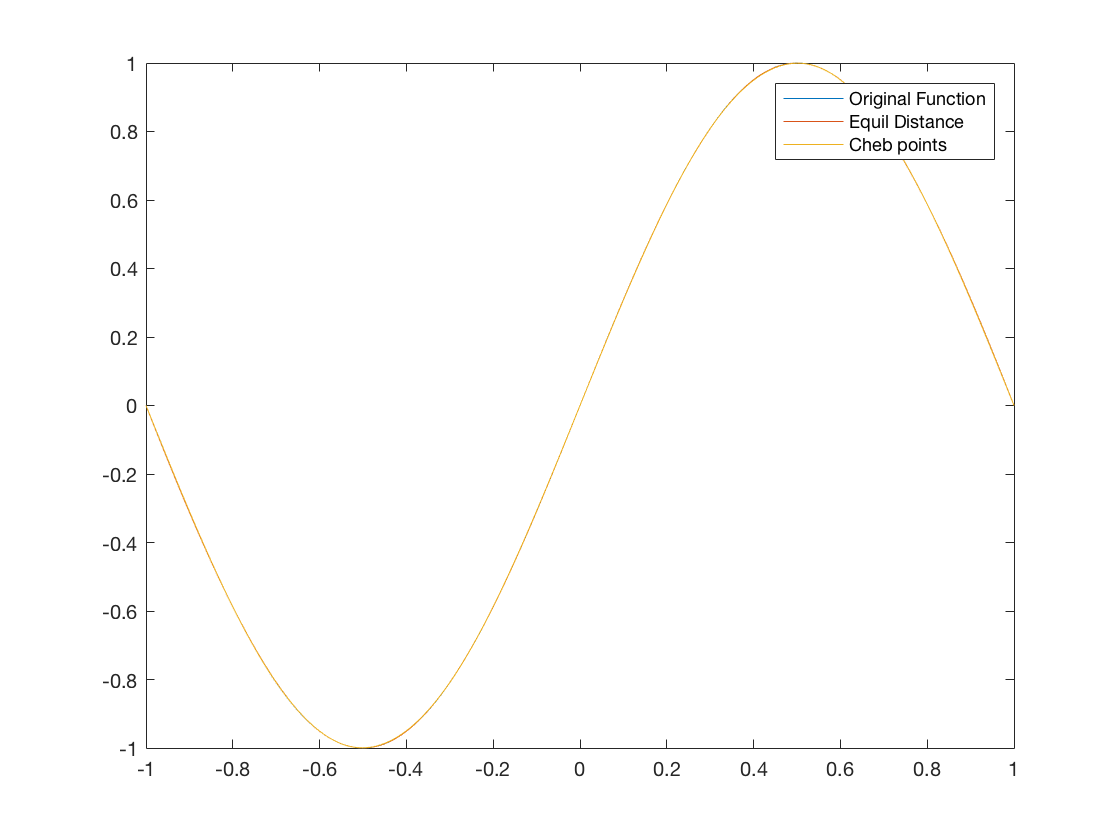
\includegraphics[scale = 0.3]{e11.png}

\subsection{• $f(x)=\frac{1}{1+25x^{2}}$}
\subparagraph{• Equidistant}
\subparagraph{• Chebyshev points}
\subsection{• $f(x)=\mid x\mid$}
\subparagraph{• Equidistant}
\subparagraph{• Chebyshev points}
\section{Question 5}
\subsection{Question 5a}
Let $x = tan(\theta)$, then\\
\centerline{$\frac{dx}{d\theta} = sec^{2}\theta$}\\
Then\\
\centerline{$dx = sec^{2}\theta d\theta$}\\
Then\\
\centerline{$\int\frac{4}{1+x^2}dx$ = $\int\frac{4}{1+tan^2(\theta)}sec^{2}\theta d\theta$}\\
Since\\
\centerline{$1+tan^2(\theta) = sec^{2}(\theta)$}\\
Then\\
\centerline{$\int\frac{4}{1+x^2}dx$ = $\int 4\;d\theta$ = $4\;\theta + C$, where $C$ is a constant}\\
Since we have set $x = tan(\theta)$, then $\theta$ = $arctan(x)$\\
Then we have \\
\centerline{$\int\frac{4}{1+x^2}dx$ = $4arctan(x)$ + C}\\
Then $\int_{0}^{1}\frac{4}{1+x^2}dx$ = $\pi$
\subsection{Question 5b}
\paragraph{• Gauss-Legendre Quadrature}\mbox{}\\
When using Gauss-Legendre Quadrature, $x_{i}'s$ are\\\\
\centerline{$x_{1} = 0.0338,x_{2}= 0.1694,x_{3}= 0.3807,x_{4}=0.6193,x_{5}=0.8306,x_{6}= 0.9662$}\\\\
And the wrights are\\\\
\centerline{$w_{1}=0.0857,w_{2}=0.1804,w_{3}=0.2340,w_{4}=0.2340,w_{5}=0.1804,w_{6}=0.0857$}\\\\
The value of the quadrature is approximated to be $\textbf{3.141592611187587}$.
\paragraph{• Composite Trapezoidal Rule}\mbox{}\\
For Gauss-Legendre Quadrature, the number of function evaluations is 6. To have the same number of function evaluations for composite trapezoidal rule, we set the number of subinterval to be 5. Then the value of the quadrature is approximated to be $\textbf{3.134926113810990}$.\\\\\\
Comparing between Gauss-Legendre Quadrature and the Composite Trapezoidal Rule, we can see that the integral approximated by Gauss-Legendre Quadrature is closer to the actual integral of the function. As we can see here, with the same number of function evaluations, Gauss-Legendre has higher accuracy than Composite Trapezoidal Rule for integral problems.
\section{Question 6}
\centerline{$\frac{Q(n)-Q(2n)}{Q(2n)-Q(4n)}$ = $\frac{(\int_{a}^{b}f(x)-Q(2n))-(\int_{a}^{b}f(x)-Q(n))}{(\int_{a}^{b}f(x)-Q(4n))-(\int_{a}^{b}f(x)-Q(2n))}$}\bigskip
For composite trapezoid rule\\\\
\centerline{$E(f)$ = $-\frac{(b-a)h^{2}}{12}f''(\xi)$, where $h = \frac{b-a}{n}$, n is the number of subintervals}\\\\
Then\\\\
\centerline{$\frac{Q(n)-Q(2n)}{Q(2n)-Q(4n)}$ = $\frac{-h_{2}^{2}+h_{1}^{2}}{-h_{4}^{2}+h_{2}^{2}}$, where $h_1=\frac{b-a}{n}, h_2=\frac{b-a}{2n}, h_4=\frac{b-a}{4n}$}\\\\
Therefore,\\\\
\centerline{$\frac{Q(n)-Q(2n)}{Q(2n)-Q(4n)} \to 4$, when $n \to \infty$}
\section{Question 7}
For Simpson's rule,\\\\
\centerline{$\int_{a}^{b}f(x)$ $\approx$ $\frac{b-a}{6}(f(a)+4f(\frac{a+b}{2})+f(b))$}\\\\
Then for composite Simpson's rule, we have:\\\\
\centerline{$\int_{a}^{b}f(x)$ $\approx$ $\frac{h}{3}(f_0+4f_1+2f_2+4f_3+....+2f_{n-2}+4f_{n-1}+f_n)$ }\\\\
\centerline{$\int_{a}^{b}f(x)$ $\approx$ $\frac{h}{3}(f(x_{0})+2\sum_{j=1}^{\frac{n}{2}-1}f(x_{2j})+4\sum_{j=1}^{\frac{n}{2}}f(x_{2j-1})+f(x_{n}))$}\\\\
For the error analysis, let $n = 2M$, then we have\\\\
%\centerline{$S$ = $\frac{h}{3}(f(x_{a})+f(x_{b}))+\frac{2h}{3}\sum_{j=1}^{M-1}f(x_{2j})+\frac{4h}{3}\sum_{j=1}^{M}f(x_{2j-1})$}\\\\
%\centerline{$\int_{a}^{b}f(x)$ = $S$ + $E_{s}$, where $E_{s}$ is the error term}\\\\
%Then\\\\
%\centerline{$\int_{a}^{b}f(x)$ - $S$ = $E_{s}$}
\centerline{$E(f)$ = $\int_{a}^{b}(f(x)-s(x))dx$}\\\\
\centerline{$E(f)$ = $\int_{a}^{b}\frac{f^{n+1}(\xi)}{(n+1)!}\prod(x-x_{i})dx$}\\\\
Then\\\\
\centerline{$E(f)$ = $\frac{f^{n+1}(\xi)}{(n+1)!}\int_{a}^{b}\prod(x-x_{i})dx$, for some $a<\xi<b$}\\\\
For Simpson's Rule, we have:\\\\
\centerline{$\prod(x-x_{i})$ = $(x-a)(x-\frac{a+b}{2})^{2}(x-b)$}\\\\
Therefore, on one subinterval, we have error $O(h^{5})$\\\\
When having composite Simpson's rule on the entire interval, we have the error being\\\\
\centerline{$O(h^{4})$}\\\\
Since we loss one order of accuracy from local to global.

\end{document}
